\section{Creating a new project}
To make some test recordings we first create a new project. Start Traverso and select ``New\dots''. Enter a name, set the number of sheets to 1, the number of tracks to 2, and leave the rest empty. Then press ``OK'' to create the project and show it's first sheet. Note: All recorded audio data will be stored in \texttt{project\_dir/project\_name/audiosources}, so if you followed our advice and selected a project directory on a pratition with lots of free space, you shouldn't run out of disk space now.

\section{Setting up the driver}
To set up the driver backend, open the preferences dialog by clicking ``Settings $\rightarrow$ Preferences\dots'' (\FigB\ \ref{fig_driversettings}). Which driver is appropriate for your system is described in chapter \ref{sect_setup}. In the driver configuration one can choose the sampling rate, and Traverso always uses the sampling rate of the driver backend for its recordings. Traverso's audio engine works entirely in 32 bit floating point precision, and you can chose from the menu ``Settings $\rightarrow$ Recording file format'' whether the data should be stored in a standard Wave format, in Wave-64, or in FLAC. The bit resolution will always be 32~bit floating point.

\begin{figure}
 \centering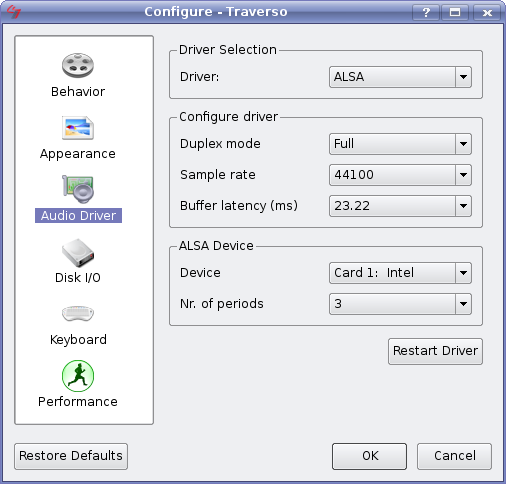
\includegraphics[width=0.75\textwidth]{images/driversettings.png}
 \caption{In ``Settings $\rightarrow$ Preferences\dots'', all driver related parameters can be set.}
 \label{fig_driversettings}
\end{figure}

\section{Recording}
Make sure a sound source is connected to the line-in bus of your sound card, and also make sure it really is playing back. In Traverso hit \sact{B} on the first track and select ``Capture 1'' as input bus, then hit \sact{A} to arm the first track. As soon as the track is armed, you should see the VUMeter indicating an input signal on Capture1. If not, the problem is most probably to be searched outside of Traverso. If you are sure your cable connections are correct, open KMix or a similar mixer applet to configure your sound card. As shown in \FigT\ \ref{fig_kmix01}, the Line and Capture channels had to be armed and un-muted on our test system before the line-in signal got through to Traverso.

\begin{figure}
 \centering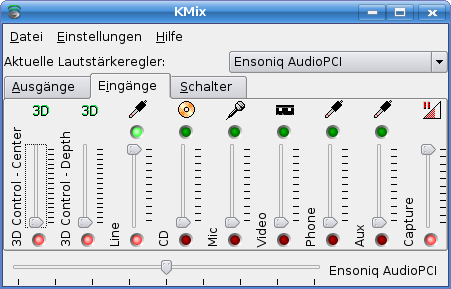
\includegraphics[width=0.8\textwidth]{images/kmix01.png}
 \caption{KMix can be used to configure the sound card. Make sure the correct input channels (Line and Capture) are un-muted and set for recording (green and red buttons).}
 \label{fig_kmix01}
\end{figure}

When you are ready to record, press the \texttt{Record} button in the title bar or hit CTRL+\sact{SPACE} to start the recording, and hit \sact{SPACE} to stop recording. That's it. In order to rehearse the recording, place the work cursor before the newly recorded clips, and press \sact{SPACE} to start playback. Once you have finished recording a track, don't forget to unarm it by pressing \sact{A}, or unarm all armed tracks at once by hitting \dact{A}.

